\def\thoigian{4}
\section
[Giải hệ hai phương trình bậc nhất hai ẩn]
{GIẢI HỆ HAI PHƯƠNG TRÌNH BẬC NHẤT HAI ẨN}

\subsection{Mục tiêu}

\paragraph{Về kiến thức, kĩ năng}

\begin{itemize}
    \item Giải hệ hai phương trình bậc nhất hai ẩn bằng phương pháp thế và phương pháp cộng đại số. 
    \item Tìm nghiệm của hệ hai phương trình bậc nhất hai ẩn bằng máy tính cầm tay (MTCT). 
\end{itemize}

\paragraph{Về năng lực}

\begin{itemize}
    \item Rèn luyện các năng lực toán học, nói riêng là năng lực tư duy và lập luận toán học, năng lực sử dụng công cụ và phương tiện học toán. 
    \item Bồi dưỡng hứng thú học tập, ý thức làm việc nhóm, ý thức tìm tòi, khám phá và sáng tạo cho HS. 
\end{itemize}

\paragraph{Về phẩm chất}

\begin{itemize}
    \item Góp phần giúp HS rèn luyện và phát triển các phẩm chất tốt đẹp (yêu nước, nhân ái, chăm chỉ, trung thực, trách nhiệm):
    \begin{itemize}
        \item Tích cực phát biểu, xây dựng bài và tham gia các hoạt động nhóm;
        \item Có ý thức tích cực tìm tòi, sáng tạo trong học tập; phát huy điểm mạnh, khắc phục các điểm yếu của bản thân. 
    \end{itemize}
\end{itemize}

\subsection{Thiết bị dạy học và học liệu}

\paragraph{Giáo viên}

\begin{itemize}
    \item Giáo án, bảng phụ, máy chiếu (nếu có), phiếu học tập, … 
\end{itemize}

\paragraph{Học sinh}

\begin{itemize}
    \item SGK, vở ghi, dụng cụ học tập, máy tính cầm tay. 
\end{itemize}

\subsection{Tiến trình dạy học}

Bài học này dạy trong 04 tiết: 
\begin{itemize}
    \item Tiết 1: Mục 1. Phương pháp thế.
    \item Tiết 2: Mục 2. Phương pháp cộng đại số.
    \item Tiết 3: Mục 3. Sử dụng MTCT tìm nghiệm của hệ hai phương trình bậc nhất hai ẩn.
    \item Tiết 4: Chữa bài tập. 
\end{itemize}

\subsubsection{Phương pháp thế}

\paragraph{Hoạt động khởi động}

\muctieu

\begin{itemize}
    \item Gợi động cơ, tạo tình huống có vấn đề về việc giải hệ hai phương trình bậc nhất hai ẩn. 
\end{itemize}

\noidungsanpham

\begin{modau}
    Một mảnh vườn được đánh thành nhiều luống, mỗi luống trồng cùng một số cây cải bắp. Hãy tính số cây cải bắp được trồng trên mảnh vườn đó, biết rằng:
    \begin{itemize}
    \item Nếu tăng thêm 8 luống, nhưng mỗi luống trồng ít đi 3 cây cải bắp thì số cải bắp của cả vườn sẽ ít đi 108 cây;
    \item Nếu giảm đi 4 luống, nhưng mỗi luống trồng tăng thêm 2 cây thì số cải bắp cả vườn sẽ tăng thêm 64 cây.
    \end{itemize}
\end{modau}

\tochucthuchien

\begin{tcth}
    \buocmot
    \item GV yêu cầu HS đọc nội dung của Tình huống mở đầu. 
    \buochai
    \item HS suy nghĩ về tình huống mở đầu và nảy sinh nhu cầu tìm hiểu cách giải hệ hai phương trình bậc nhất hai ẩn.
    \buocba
    \item HS trả lời câu hỏi (không yêu cầu trả lời chính xác).
    \buocbon
    \item GV giới thiệu bài học mới về giải phương trình bậc nhất hai ẩn.
\end{tcth}

\paragraph{Hoạt động hình thành kiến thức}

\muctieu

\begin{itemize}
    \item HS biết cách giải hệ hai phương trình bậc nhất hai ẩn bằng phương pháp thế. 
\end{itemize}

\noidungsanpham

\begin{ttkp}
    \textbf{Làm quen với phương pháp thế}\\
    \textbf{HĐ1:} 
    Cho hệ phương trình $\heva{&x+y=3\\&2x-3y=1}$. Giải hệ phương trình theo hướng dẫn sau:
    \begin{listEX} 
        \item Từ phương trình thứ nhất, biểu diễn y theo x rồi thế vào phương trình thứ hai để được một phương trình với một ẩn x. Giải phương trình một ẩn đó để tìm giá trị của x. 
        \item Sử dụng giá trị tìm được của x để tìm giá trị của y rồi viết nghiệm của hệ phương trình đã cho. 
    \end{listEX}
    %%%
    \doicot
    %%%
    \textbf{HĐ1:}
    \begin{listEX}
        \item Từ phương trình thứ nhất, ta có $x=3-y$.\\
        Thế vào phương trình thứ hai ta được $2(3-y)-3y=1$, suy ra $y=1$.
        \item Với $y=1$ thì $x=3-1=2$.\\
        Vậy nghiệm của hệ đã cho là $(2;1)$.
    \end{listEX} 
\end{ttkp}

\begin{vidu}
    Giải hệ phương trình $\heva{&2x-y=3\\&x+2y=4}$ bằng phương pháp thế.
    %%%
    \doicot
    %%%
    Từ phương trình thứ nhất của hệ ta có $y = 2x - 3$. Thế vào phương trình thứ hai của hệ, ta được $x + 2(2x - 3) = 4$ hay $5x - 6 = 4$, suy ra $x = 2$.\\
    Từ đó $y = 2 \cdot 2 - 3 = 1$. Vậy hệ phương trình đã cho có nghiệm là $(2; 1)$.
\end{vidu}

\tochucthuchien

\begin{tcth}[ttkp]
    \buocmot
    \item GV hướng dẫn HS thực hiện lần lượt các yêu cầu trong HĐ1.
    \buochai
    \item HS thực hiện cá nhân HĐ1. 
    \buocba
    \item GV yêu cầu HS nêu cách giải hệ phương trình bậc nhất hai ẩn bằng phương pháp thế.
    \item HS giơ tay phát biểu.
    \buocbon
    \item GV nhận xét, kết luận và phân tích cách giải hệ phương trình bằng phương pháp thế.
    \item GV viết bảng hoặc trình chiếu nội dung trong Khung kiến thức. 
    \begin{kttt}
        \textbf{Cách giải hệ phương trình bằng phương pháp thế:}
        \begin{cacbuoc}
            \item Từ một phương trình của hệ, biểu diễn một ẩn theo ẩn kia rồi thế vào phương trình còn lại của hệ để được phương trình chỉ còn chứa một ẩn.
            \item Giải phương trình một ẩn vừa nhận được, từ đó suy ra nghiệm của hệ đã cho.
        \end{cacbuoc}
    \end{kttt}
\end{tcth}

\begin{tcth}[vidu=1]
    \buocmot
    \item GV yêu cầu HS hoạt động cá nhân trong 3 phút để giải hệ phương trình của Ví dụ 1 bằng phương pháp thế.
    \buochai
    \item HS thực hiện theo hướng dẫn của GV.
    \buocba
    \item HS giơ tay phát biểu.
    \buocbon
    \item GV chữa bài và hướng dẫn chi tiết các bước làm cho HS.
\end{tcth}

\paragraph{Hoạt động luyện tập}

\muctieu

\begin{itemize}
    \item Củng cố kĩ năng giải hệ hai phương trình bậc nhất hai ẩn bằng phương pháp thế.
\end{itemize}

\noidungsanpham

\begin{luyentap}
    Giải các hệ phương trình sau bằng phương pháp thế:
    \begin{listEX}
        \item $\heva{&x - 3y = 2 \\ &-2x + 5y = 1}$;
        \item $\heva{&4x + y = -1 \\ &7x + 2y = -3}$.
    \end{listEX}
    %%%
    \doicot
    %%%
    \huongdan
    \begin{listEX}
        \item Kết quả là $(-13 ; -5)$.\\
        Tình huống biểu diễn $x$ theo $y$; 
        \item Kết quả là $(1 ; -5)$.\\
        Tình huống biểu diễn $y$ theo $x$. 
    \end{listEX}
\end{luyentap}

\begin{vidu}
    Giải hệ phương trình $\heva{&x - y = -2 \\ &2x - 2y = 8}$ bằng phương pháp thế.
    %%%
    \doicot
    %%%
    Từ phương trình thứ nhất ta có $x = y - 2$. Thế vào phương trình thứ hai, ta được $2(y - 2) - 2y = 8$ hay $0y - 4 = 8$. \quad (1)\\
    Do không có giá trị nào của $y$ thoả mãn hệ thức (1) nên hệ phương trình đã cho vô nghiệm.
\end{vidu}

\begin{luyentap}
    Giải hệ phương trình $\heva{&-2x + y = 3 \\ &4x - 2y = -4}$ bằng phương pháp thế.
    %%%
    \doicot
    %%%
    \huongdan\\
    Biểu diễn $y$ theo $x$ từ phương trình thứ nhất, kết quả hệ vô nghiệm.
\end{luyentap}

\begin{vidu}
    Giải hệ phương trình $\heva{&-x + y = -2 \\ &3x - 3y = 6}$ bằng phương pháp thế.
    %%%
    \doicot
    %%%
    Từ phương trình thứ nhất ta có $y = x - 2$. \quad (2)\\
    Thế vào phương trình thứ hai, ta được $3x - 3(x - 2) = 6$ hay $0x = 0$. \quad (3)\\
    Ta thấy mọi giá trị của $x$ đều thoả mãn hệ thức (3).\\
    Với giá trị tuỳ ý của $x$, giá trị tương ứng của $y$ được tính bởi (2).\\
    Vậy hệ phương trình đã cho có nghiệm là $(x; x - 2)$ với $x \in \mathbb{R}$ tuỳ ý.
\end{vidu}

\begin{luyentap}
    Giải hệ phương trình $\heva{&x + 3y = -1 \\ &3x + 9y = -3}$ bằng phương pháp thế.
    %%%
    \doicot
    %%%
    \huongdan\\
    Hệ có nghiệm là $\left(x;\dfrac{-x-1}{3}\right)$, với $x\in\mathbb{R}$ tuỳ ý.
\end{luyentap}

\tochucthuchien

\begin{tcth}[luyentap=1]
    \buocmot
    \item GV yêu cầu HS làm việc cá nhân trong 4 phút.
    \item GV cần lưu ý cho HS, có thể chọn cách biểu diễn $x$ theo $y$ hoặc biểu diễn $y$ theo $x$. 
    \buochai
    \item HS thực hiện cá nhân Luyện tập 1. 
    \buocba
    \item GV gọi hai HS lên bảng trình bày lời giải.
    \buocbon
    \item GV chữa bài và hướng dẫn chi tiết các bước làm cho HS.
\end{tcth}

\begin{tcth}[vidu=2]
    \buocmot
    \item GV hướng dẫn HS thực hiện Ví dụ 2. 
    \item GV lưu ý cho HS: Nếu từ hệ đã cho, bằng phương pháp thế ta dẫn đến một phương trình vô nghiệm thì hệ đã cho vô nghiệm. 
    \buochai
    \item HS làm việc dưới sự hướng dẫn của GV. 
    \buocba
    \item HS làm bài vào vở.
    \buocbon
    \item GV chữa bài và hướng dẫn chi tiết các bước làm cho HS.
\end{tcth}

\begin{tcth}[luyentap=2]
    \buocmot
    \item GV yêu cầu HS làm việc cá nhân trong 3 phút.
    \buochai
    \item HS thực hiện cá nhân Luyện tập 2. 
    \buocba
    \item GV gọi HS lên bảng trình bày lời giải.
    \buocbon
    \item GV chữa bài và hướng dẫn chi tiết các bước làm cho HS.
\end{tcth}

\begin{tcth}[vidu=3]
    \buocmot
    \item GV hướng dẫn HS làm Ví dụ 3.
    \item GV lưu ý cho HS: Nếu từ hệ đã cho ta dẫn đến một phương trình nghiệm đúng với mọi $x$, $y$ thì hệ đã cho có vô số nghiệm. 
    \buochai
    \item HS làm việc dưới sự hướng dẫn của GV. 
    \buocba
    \item HS làm bài vào vở.
    \buocbon
    \item GV chữa bài và hướng dẫn chi tiết các bước làm cho HS.
\end{tcth}

\begin{tcth}[luyentap=3]
    \buocmot
    \item GV yêu cầu HS làm việc cá nhân thực hiện các câu của Luyện tập 3.  
    \buochai
    \item HS thực hiện cá nhân Luyện tập 3. 
    \buocba
    \item GV gọi HS lên bảng trình bày lời giải.
    \buocbon
    \item GV chữa bài và hướng dẫn chi tiết các bước làm cho HS.
\end{tcth}

\paragraph{Hoạt động vận dụng}

\muctieu

\begin{itemize}
    \item Giúp học sinh biết vận dụng kiến thức về hệ hai phương trình bậc nhất hai ẩn để trả lời câu hỏi của bài toán trong Tình huống mở đầu.
\end{itemize}

\noidungsanpham

\begin{vandung}
    Xét bài toán trong \textit{tình huống mở đầu}. Gọi $x$ là số luống trong vườn, $y$ là số cây cải bắp trồng ở mỗi luống ($x, y \in \mathbb{N}^*$).
    \begin{listEX}
        \item Lập hệ phương trình đối với hai ẩn $x$, $y$.
        \item Giải hệ phương trình nhận được ở câu a) để tìm câu trả lời cho bài toán.
    \end{listEX}
    %%%
    \doicot
    %%%
    \huongdan
    \begin{listEX}
        \item $\heva{&3x-8y=84\\&x-2y=36}$.
        \item Nghiệm của phương trình trên là $(60;12)$.\\
        Số cây bắp cải được trồng trên mảnh vườn đó là:
        $$60\cdot12=720\text{ (cây)}.$$
    \end{listEX}
\end{vandung}

\paragraph{Tổng kết và hướng dẫn công việc ở nhà}

GV tổng kết lại nội dung bài học và dặn dò công việc ở nhà cho HS:

\begin{itemize}
    \item  GV tổng kết lại các kiến thức trọng tâm của bài học: Cách giải hệ phương trình bằng phương pháp thế. 
    \item Nhắc HS về nhà ôn tập các nội dung đã học. 
    \item Giao cho HS làm bài tập trong SGK: Bài 1.6.
\end{itemize}

\subsubsection{Phương pháp cộng đại số}

\paragraph{Hoạt động hình thành kiến thức}

\muctieu

\begin{itemize}
    \item HS biết cách giải hệ hai phương trình bậc nhất hai ẩn bằng phương pháp cộng đại số. 
\end{itemize}

\noidungsanpham

\begin{ttkp}
    \textbf{HĐ2:}\\
    Cho hệ phương trình $\heva{&2x + 2y = 3 \\ &x - 2y = 6}$. Ta thấy hệ số của $y$ trong hai phương trình là hai số đối nhau (tổng của chúng bằng 0). Từ đặc điểm đó, hãy giải hệ phương trình đã cho theo hướng dẫn sau:
    \begin{listEX}
        \item Cộng từng vế của hai phương trình trong hệ để được phương trình một ẩn $x$. Giải phương trình này để tìm $x$.
        \item Sử dụng giá trị $x$ tìm được, thay vào một trong hai phương trình của hệ để tìm giá trị của $y$ rồi viết nghiệm của hệ phương trình đã cho.
    \end{listEX}
    %%%
    \doicot
    %%%
    \textbf{HĐ2:}\\
    \huongdan\\
    \begin{listEX}
        \item Cộng từng vế của hai phương trình ta được: $3x = 9$ nên $x = 3$.
        \item Với $x = 3$ ta có $3 - 2y = 6$ nên $y = \dfrac{-3}{2}$.\\
        Vậy nghiệm của hệ đã cho là $\left(3;\dfrac{-3}{2}\right)$.
    \end{listEX}
\end{ttkp}

\begin{vidu}
    Giải hệ phương trình $\heva{&-2x + 5y = 12 \\ &2x + 3y = 4}$ bằng \\
    phương pháp cộng đại số.
    %%%
    \doicot
    %%%
    Cộng từng vế hai phương trình ta được $8y = 16$, suy ra $y = 2$.\\
    Thế $y = 2$ vào phương trình thứ hai ta được $2x + 3 \cdot 2 = 4$, hay $2x = -2$, suy ra $x = -1$.\\
    Vậy hệ phương trình đã cho có nghiệm là $(-1; 2)$.
\end{vidu}

\begin{vidu}
    Giải hệ phương trình $\heva{&5x - 7y = 9 \\ &5x - 3y = 1}$ bằng phương pháp cộng đại số.
    %%%
    \doicot
    %%%
    Trừ từng vế của hai phương trình, ta được $(5x - 5x) + (-7y + 3y) = 9 - 1$ hay $-4y = 8$, suy ra $y = -2$.\\
    Thế $y = -2$ vào phương trình thứ nhất, ta được $5x - 7 \cdot (-2) = 9$ hay $5x + 14 = 9$, suy ra $x = -1$.\\
    Vậy hệ phương trình đã cho có nghiệm là $(-1; -2)$.
\end{vidu}

\tochucthuchien

\begin{tcth}[ttkp]
    \buocmot
    \item GV hướng dẫn HS thực hiện lần lượt các yêu cầu trong HĐ2.
    \buochai
    \item HS thực hiện cá nhân HĐ2.
    \buocba
    \item GV yêu cầu HS nêu cách giải hệ hai phương trình bậc nhất hai ẩn bằng phương pháp cộng đại số.
    \buocbon
    \item GV viết bảng hoặc trình chiếu nội dung trong Khung kiến thức.
    \begin{kttt}
        \textbf{Cách giải hệ phương trình bằng phương pháp cộng đại số:}\\
        Để giải một hệ hai phương trình bậc nhất hai ẩn có hệ số của cùng một ẩn nào đó trong hai phương trình bằng nhau hoặc đối nhau, ta có thể làm như sau:
        \begin{cacbuoc}
            \item Cộng hay trừ từng vế của hai phương trình trong hệ để được phương trình chỉ còn chứa một ẩn.
            \item Giải phương trình một ẩn vừa nhận được, từ đó suy ra nghiệm của hệ phương trình đã cho.
        \end{cacbuoc}
    \end{kttt}
\end{tcth}

\begin{tcth}[vidu=4]
    \buocmot
    \item GV hướng dẫn HS giải hệ phương trình của Ví dụ 4 bằng phương pháp cộng đại số.
    \item GV cần lưu ý cho HS trường hợp hệ số của $x$ đối nhau: Cộng từng vế hai phương trình.
    \buochai
    \item HS thực hiện dưới sự hướng dẫn của GV. 
    \buocba
    \item HS làm bài vào vở.
    \buocbon
    \item GV nhận xét, kết luận và phân tích cách giải hệ phương trình bằng phương pháp cộng đại số.
\end{tcth}

\begin{tcth}[vidu=5]
    \buocmot
    \item GV hướng dẫn HS giải hệ phương trình của Ví dụ 5 bằng phương pháp cộng đại số.
    \item GV cần lưu ý cho HS trường hợp hệ số của $x$ bằng nhau: Trừ từng vế hai phương trình.
    \buochai
    \item HS thực hiện dưới sự hướng dẫn của GV. 
    \buocba
    \item HS làm bài vào vở.
    \buocbon
    \item GV nhận xét, kết luận và phân tích cách giải hệ phương trình bằng phương pháp cộng đại số.
\end{tcth}

\paragraph{Hoạt động luyện tập}

\muctieu

\begin{itemize}
    \item Củng cố kĩ năng giải hệ hai phương trình trình bậc nhất hai ẩn bằng phương pháp cộng đại số.
\end{itemize}

\noidungsanpham

\begin{luyentap}
    Giải các hệ phương trình sau bằng phương pháp cộng đại số:
    \begin{listEX}
        \item $\heva{&-4x + 3y = 0 \\ &4x - 5y = -8;}$;
        \item $\heva{&4x + 3y = 0 \\ &x + 3y = 9.}$
    \end{listEX}
    %%%
    \doicot
    %%%
    \textit{Hướng dẫn}:
    \begin{listEX}
        \item Nghiệm của hệ là $(3;4)$;
        \item Nghiệm của hệ là $(-3;4)$.
    \end{listEX}
\end{luyentap}

\begin{vidu}
    Giải hệ phương trình $\heva{&3x + 2y = 7 \\ &2x - 3y = -4}$ bằng phương pháp cộng đại số.
    %%%
    \doicot
    %%%
    Nhân hai vế của phương trình thứ nhất với 3 và nhân hai vế của phương trình thứ hai với 2, ta được:
    $$\heva{&9x + 6y = 21 \\ &4x - 6y = -8.}$$
    Cộng từng vế hai phương trình của hệ mới, ta được $13x = 13$ hay $x = 1$.\\
    Thế $x = 1$ vào phương trình thứ nhất của hệ đã cho, ta có $3 \cdot 1 + 2y = 7$, suy ra $y = 2$.\\
    Vậy hệ phương trình đã cho có nghiệm là $(1; 2)$.
\end{vidu}

\begin{luyentap}
    Giải hệ phương trình $\heva{&4x + 3y = 6 \\ &-5x + 2y = 4}$ bằng phương pháp cộng đại số.
    %%%
    \doicot
    %%%
    \textit{Hướng dẫn}:\\
    Nghiệm của hệ là $(0;2)$.
\end{luyentap}

\begin{vidu}
    Giải hệ phương trình $\heva{&3x - 5y = 2 \\ &-6x + 10y = -4}$ bằng phương pháp cộng đại số.
    %%%
    \doicot
    %%%
    Chia hai vế của phương trình thứ hai cho 2, ta được hệ $$\heva{&3x - 5y = 2 \\ &-3x + 5y = -2.}$$
    Cộng từng vế hai phương trình của hệ mới ta có $0x + 0y = 0$. Hệ thức này luôn thoả mãn với các giá trị tuỳ ý của $x$ và $y$.\\
    Với giá trị tuỳ ý của $x$, giá trị của $y$ được tính nhờ hệ thức $3x - 5y = 2$, suy ra $y = \dfrac{3}{5}x - \dfrac{2}{5}$.\\
    Vậy hệ phương trình đã cho có nghiệm là\\$\left( x; \dfrac{3}{5}x - \dfrac{2}{5} \right)$ với $x \in \mathbb{R}$.
\end{vidu}

\tochucthuchien

\begin{tcth}[luyentap=4]
    \buocmot
    \item GV chia lớp thành hai nhóm tương ứng với hai dãy bàn, mỗi cá nhân trong dãy làm một ý a hoặc b trong 3 phút.
    \buochai
    \item HS làm việc dưới sự hướng dẫn của GV. 
    \buocba
    \item GV gọi hai HS đại diện hai dãy lên bảng trình bày lời giải.
    \buocbon
    \item GV nhận xét và đưa ra đáp án chính xác.
\end{tcth}

\begin{tcth}[vidu=6]
    \buocmot
    \item GV hướng dẫn HS giải hệ phương trình của Ví dụ 6 bằng phương pháp cộng đại số. 
    \item GV lưu ý HS: 
    \begin{chuy}
        Trường hợp trong hệ phương trình đã cho không có hai hệ số của cùng một ẩn bằng nhau hay đối nhau, ta có thể đưa về trường hợp đã xét bằng cách nhân hai vế của mỗi phương trình với một số thích hợp (khác $0$).
    \end{chuy}
    \buochai
    \item HS làm việc dưới sự hướng dẫn của GV. 
    \buocba
    \item HS làm bài vào vở.
    \buocbon
    \item GV nhận xét và đưa ra đáp án chính xác.
\end{tcth}

\begin{tcth}[luyentap=5]
    \buocmot
    \item  GV yêu cầu HS làm việc cá nhân.
    \buochai
    \item HS tự làm bài tại lớp.
    \buocba
    \item GV gọi HS lên bảng trình bày lời giải.
    \buocbon
    \item GV nhận xét và đưa ra đáp án chính xác.
\end{tcth}

\begin{tcth}[vidu=6]
    \buocmot
    \item  GV hướng dẫn HS giải hệ phương trình của Ví dụ 7 bằng phương pháp cộng đại số trong trường hợp hệ có vô số nghiệm.
    \buochai
    \item HS thực hiện dưới sự hướng dẫn của GV. 
    \buocba
    \item HS làm bài vào vở.
    \buocbon
    \item GV nhận xét và đưa ra đáp án chính xác.
\end{tcth}

\paragraph{Hoạt động vận dụng}

\muctieu

\begin{itemize}
    \item Giúp HS lập được hệ phương trình dưới sự hướng dẫn của GV và củng cố cách giải hệ để trả lời câu hỏi của bài toán vận dụng.
\end{itemize}

\noidungsanpham

\begin{vandung}
    Tổng số học sinh khối $8$ và khối $9$ của một trường là $660$ em, trong đó có $413$ em là học sinh giỏi. Biết rằng số học sinh giỏi khối $8$ chiếm tỉ lệ $60 \%$ số học
    sinh của khối $8$, số học sinh giỏi khối $9$ chiếm tỉ lệ $65 \%$ số học sinh khối $9$.
    \begin{listEX}
        \item Gọi $x$ và $y$ lần lượt là số học sinh của khối $8$ và khối $9$ ($x$, $y$ $\in\mathbb{N}^*$, $x$, $y< 660$). Lập hệ phương trình đối với hai ẩn $x$ và $y$.
        \item Giải hệ phương trình nhận được ở câu a để tìm số học sinh của mỗi khối.
    \end{listEX}
    %%%
    \doicot
    %%%
    \begin{listEX}
        \item $\heva{&x+y=600\\&0{,}6x+0{,}65y=413.}$
        \item Nghiệm của hệ phương trình là $(300;340)$.\\
        Vậy trường có $320$ học sinh khối $8$ và $340$ học sinh khối $9$.
    \end{listEX}
\end{vandung}

\tochucthuchien

\begin{tcth}
    \buocmot
    \item GV đưa ra bài toán vận dụng.
    \item GV hướng dẫn HS từng bước để lập được hệ phương trình, sau đó yêu cầu HS vận dụng phương pháp giải hệ hai phương trình đã được học, để giải quyết vấn đề của bài vận dụng.
    \buochai
    \item HS làm việc dưới sự hướng dẫn của GV. 
    \buocba
    \item HS giơ tay lên bảng làm bài.
    \buocbon
    \item GV nhận xét và đưa ra đáp án chính xác.
\end{tcth}

\paragraph{Tổng kết và hướng dẫn công việc về nhà}

GV tổng kết lại nội dung bài học và dặn dò công việc ở nhà cho HS:
\begin{itemize}
    \item GV tổng kết lại các kiến thức trọng tâm của bài học: Cách giải hệ hai phương trình bậc nhất hai ẩn bằng phương pháp cộng đại số. 
    \item Làm Luyện tập 6 SGK trang 14. 
    \item Giao cho HS làm các bài tập sau trong SGK: Bài 1.7; 1.8; 1.9 và 1.10.
\end{itemize}

\subsubsection{Sử dụng máy tính cầm tay để tìm nghiệm của hệ hai phương trình bậc nhất hai ẩn}

\paragraph{Hoạt động hình thành kiến thức}

\muctieu

\begin{itemize}
    \item HS biết cách tìm nghiệm của hệ hai phương trình bậc nhất hai ẩn bằng MTCT. 
\end{itemize}

\noidungsanpham

\begin{dhnh}
    Muốn tìm nghiệm của hệ hai phương trình bậc nhất hai ẩn bằng máy tính cầm tay (MTCT), chúng ta cần sử dụng loại máy có chức năng này (thường có phím MODE).\\
    Trước hết ta phải viết hệ phương trình cần tìm nghiệm dưới dạng:
    $$\heva{&a_1x + b_1y = c_1 \\ &a_2x + b_2y = c_2.}$$
    Chẳng hạn để tìm nghiệm của hệ 
    $$\heva{&2x + 3y - 4 = 0 \\ &5x + 6y - 7 = 0,}$$
    Ta viết nó dưới dạng 
    $$\heva{&2x + 3y = 4 \\ &5x + 6y = 7.}$$
    Khi đó, ta có $a_1 = 2$, $b_1 = 3$, $c_1 = 4$; $a_2 = 5$, $b_2 = 6$ và $c_2 = 7$. Lần lượt thực hiện các bước sau (với máy tính thích hợp):
    \begin{cacbuoc}
        \item Vào chức năng giải hệ hai phương trình bậc nhất hai ẩn bằng cách bấm các phím \fbox{MODE} \fbox{5} \fbox{1} (xem \textit{màn hình sau bước 1}, con trỏ ở vị trí $a_1$).
        \item Nhập các số $a_1 = 2, b_1 = 3, c_1 = 4; a_2 = 5, b_2 = 6$ và $c_2 = 7$ bằng cách bấm: \\
        \fbox{2} \fbox{=} \fbox{3} \fbox{=} \fbox{4} \fbox{=} \fbox{5} \fbox{=} \fbox{6} \fbox{=} \fbox{7} \fbox{=} (xem \textit{màn hình sau bước 2}).
        \item Đọc kết quả: Sau khi kết thúc bước 2, bấm \fbox{=}, màn hình cho $x = -1$; bấm tiếp phím \fbox{=}, màn hình cho $y = 2$ (xem \textit{màn hình sau bước 3}). Ta hiểu nghiệm của hệ phương trình là $(-1; 2)$.
    \end{cacbuoc}
    %%%
    \doicot
    %%%
    \begin{cacbuoc}
        \item \hfill\par
        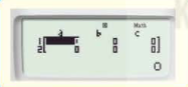
\includegraphics[width=0.8\linewidth]{imgs/9D1-2-casio-1.png}
        \item \hfill\par
        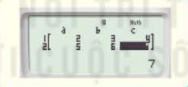
\includegraphics[width=0.8\linewidth]{imgs/9D1-2-casio-2.png}
        \item \hfill\par
        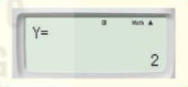
\includegraphics[width=0.8\linewidth]{imgs/9D1-2-casio-3.png}
    \end{cacbuoc}
\end{dhnh}

\tochucthuchien

\begin{tcth}
    \buocmot
    \item GV yêu cầu HS tự đọc thông tin từ phần Đọc hiểu - Nghe hiểu và thực hiện theo các bước.\\
    \textit{Lưu ý: GV hướng dẫn phù hợp với loại máy tính mà HS đang sử dụng. }
    \buochai
    \item HS đọc thông tin và thực hiện với MTCT của mình. 
    \item GV quan sát và hỗ trợ HS trong lúc thực hành. 
    \buocba
    \item HS thảo luận cách dùng MTCT.
    \buocbon
    \item GV đưa ra Chú ý:
    \begin{chuy}
        \begin{itemize}
            \item Muốn xoá số vừa mới nhập thì bấm phím \fbox{AC}; muốn thay đổi số đã nhập ở một vị trí nào đó thì di chuyển con trỏ đến vị trí đó rồi nhập số mới.
            \item Bấm phím \fbox{$\blacktriangle$} hay \fbox{$\blacktriangledown$} để chuyển đổi hiển thị các giá trị của $x$ và $y$ trong kết quả.
            \item Nếu máy báo ``Infinite Sol'' thì hệ phương trình đã cho có vô số nghiệm. Nếu máy báo ``No--Solution'' thì hệ phương trình đã cho vô nghiệm.
        \end{itemize}
    \end{chuy}
\end{tcth}

\paragraph{Hoạt động luyện tập}

\muctieu

\begin{itemize}
    \item Củng cố kĩ năng tìm nghiệm của hệ hai phương trình trình bậc nhất hai ẩn bằng MTCT.
\end{itemize}

\noidungsanpham

\begin{thuchanh}
    Dùng MTCT thích hợp để tìm nghiệm của các hệ phương trình sau:
    \begin{listEX}[2]
        \item $\heva{&2x + 3y = -4 \\ &-3x - 7y = 13;}$
        \item $\heva{&2x + 3y = 1 \\ &-x - 1,5y = 1;}$
        \item $\heva{&8x - 2y - 6 = 0 \\ &4x - y - 3 = 0.}$
    \end{listEX}
    %%%
    \doicot
    %%%
    \huongdan
    \begin{listEX}
        \item Hệ phương trình có nghiệm là $\left(\dfrac{11}{5};\dfrac{-11}{5}\right)$;
        \item Hệ phương trình vô nghiệm;
        \item Hệ phương trình có vô số nghiệm:
        $$(x;4x-3)\text{ với }x\in\mathbb{R}.$$
    \end{listEX}
\end{thuchanh}

\tochucthuchien

\begin{tcth}
    \buocmot
    \item GV tổ chức cho HS thực hành giải hệ phương trình bằng 
    \buochai
    \item HS thực hiện dưới sự hướng dẫn của GV. 
    \buocba
    \item HS giờ tay phát biểu.
    \buocbon
    \item GV nhận xét và giải đáp thắc mắc của HS. Chú ý hướng dẫn HS đưa ra dạng nghiệm tổng quát ở ý c.
\end{tcth}

\paragraph{Hoạt động vận dụng}

\muctieu

\begin{itemize}
    \item  Giúp học sinh vận dụng kiến thức về giải hệ hai phương trình bậc nhất hai ẩn để giải quyết một bài toán liên quan đến Hóa học.
\end{itemize}

\noidungsanpham

\begin{vandung}
    Thực hiện lần lượt các yêu cầu sau để tính số mililít dung dịch acid HCl nồng độ 20 \% và số mililít dung dịch acid HCl nồng độ 5 \% cần dùng để pha chế 2 lít dung dịch acid HCl nồng độ 10 \%.
    \begin{listEX}
        \item Gọi $x$ là số mililít dung dịch acid HCl nồng độ 20\%, $y$ là số mililít dung dịch acid HCl nồng độ 5\% cần lấy. Hãy biểu thị qua $x$ và $y$:
        \begin{itemize}
            \item Thể tích của dung dịch acid HCl 10\% nhận được sau khi trộn lẫn hai dung dịch acid ban đầu.
            \item Tổng số mililít acid HCl nguyên chất có trong hai dung dịch acid này.
        \end{itemize}
        \item Sử dụng kết quả ở câu a, hãy lập một hệ hai phương trình bậc nhất với hai ẩn là $x$, $y$. Giải hệ phương trình này để tính số mililít cần lấy của mỗi dung dịch acid HCl ở trên.
    \end{listEX}
    %%%
    \doicot
    %%%
    \huongdan\\
    Ta có hệ phương trình:
    $$\heva{&x+y=2000\\&\dfrac{0{,}2x+0{,}05y}{2000}}=0,1.$$
    Giải hệ phương trình trên, ta được:
    $$x=\dfrac{2000}{y};y=\dfrac{4000}{3}.$$
\end{vandung}

\begin{phieuhoctap}
	Xem Phiếu học tập 1 ở mục Phụ lục.
	%%%
	\doicot
	%%%
	\huongdan\\
	\textbf{Câu 1.} C\\
	\textbf{Câu 2.} C\\
	\textbf{Câu 3.} D\\
	\textbf{Câu 4.} A\\
	\textbf{Câu 5.} B\\
	\textbf{Câu 6.} D
\end{phieuhoctap}

\tochucthuchien

\begin{tcth}[vandung=3]
    \buocmot
    \item GV tổ chức cho HS làm việc nhóm đôi để thảo luận thực hiện nhiệm vụ của phần Vận dụng
    \buochai
    \item HS làm việc theo nhóm dưới sự hướng dẫn của GV. 
    \buocba
    \item GV gọi đại diện 2 nhóm lên bảng trình bày.
    \item Các nhóm khác nhận xét.
    \buocbon
    \item GV phân tích, nhận xét bài làm của HS.
\end{tcth}

\begin{tcth}[phieuhoctap=1]
	\buocmot
	\item HS làm theo nhóm bốn vào phiếu học tập số 1.
	\buochai
	\item HS làm việc theo nhóm dưới sự hướng dẫn của GV. 
	\buocba
	\item GV gọi đại diện các nhóm đưa ra đáp án từng câu.
	\item Các nhóm khác nhận xét.
	\buocbon
	\item GV phân tích, nhận xét câu trả lời của HS.
\end{tcth}

\subsubsection{Chữa bài tập cuối bài trong SGK}

\paragraph{Hoạt động khởi động}

\muctieu

\begin{itemize}
    \item HS nhớ lại các cách giải hệ hai phương trình bậc nhất hai ẩn đã học. 
\end{itemize}

\noidungsanpham

\begin{phieuhoctap}
	Xem Phiếu học tập 2 ở mục Phụ lục.
	%%%
	\doicot
	%%%
	\huongdan\\
	\textbf{Câu 1.} Biểu diễn, thế, một, một ẩn, nghiệm.\\
	\textbf{Câu 2.} Bằng nhau, đối nhau, cộng, trừ, một ẩn, một ẩn, nghiệm.
\end{phieuhoctap}

\tochucthuchien

\begin{tcth}
    \buocmot
    \item GV cho HS hoạt động theo cặp trong 3 phút để hoàn thành phiếu học tập số 2 trong Phụ lục.
    \buochai
    \item HS thực hiện phiếu học tập số 2. 
    \buocba
    \item HS giơ tay phát biểu.
    \item Các HS khác theo dõi bài làm, nhận xét và góp ý.
    \buocbon
    \item GV tổng kết.
\end{tcth}

\paragraph{Hoạt động luyện tập}

\muctieu

\begin{itemize}
    \item Củng cố cách giải hệ hai phương trình bậc nhất hai ẩn bằng phương pháp thế, phương pháp cộng đại số hoặc sử dụng máy tính cầm tay.
\end{itemize}

\noidungsanpham

\begin{baitap}[1.6]
    Giải các hệ phương trình sau bằng phương pháp thế:
    \begin{listEX}[2]
        \item $\heva{&x - y = 3 \\ &3x - 4y = 2;}$
        \item $\heva{&7x - 3y = 13 \\ &4x + y = 2;}$
        \item $\heva{&0,5x - 1,5y = 1 \\ &-x + 3y = 2.}$
    \end{listEX}
    %%%
    \doicot
    %%%
    \huongdan
    \begin{listEX}
    	\item $(10;7)$;
    	\item $(1;-2)$;
    	\item Vô nghiệm.
    \end{listEX}
\end{baitap}

\begin{baitap}[1.7]
    Giải các hệ phương trình sau bằng phương pháp cộng đại số:
    \begin{listEX}[2]
        \item $\heva{&3x + 2y = 6 \\ &2x - 2y = 14;}$
        \item $\heva{&0,3x + 0,5y = 3 \\ &1,5x - 2y = 1,5;}$ 
        \item $\heva{&-2x + 6y = 8 \\ &3x - 9y = -12.}$
    \end{listEX}
    %%%
    \doicot
    %%%
    \huongdan
    \begin{listEX}
    	\item $(4;-3)$;
    	\item $(5;3)$;
    	\item Vô số nghiệm: $\left(x;\dfrac{x+4}{3}\right)$ với $x\in\mathbb{R}$.
    \end{listEX}
\end{baitap}

\begin{baitap}[1.8]
    Cho hệ phương trình $\heva{&2x - y = -3 \\ &-2m^2x + 9y = 3(m + 3)}$, trong đó $m$ là số đã cho. Giải hệ phương trình trong mỗi trường hợp sau:
    \begin{listEX}[3]
        \item $m = -2$;
        \item $m = -3$;
        \item $m = 3$.
    \end{listEX}
    %%%
    \doicot
    %%%
    \huongdan
    \begin{listEX}
    	\item $\left(-\dfrac{12}{5};-\dfrac{9}{5}\right)$;
    	\item Vô nghiệm;
    	\item Vô nghiệm.
    \end{listEX}
\end{baitap}

\begin{baitap}[1.9]
    Dùng MTCT thích hợp để tìm nghiệm của các hệ phương trình sau:
    \begin{listEX}
        \item $\heva{&12x - 5y + 24 = 0 \\ &-5x - 3y - 10 = 0;}$
        \item $\heva{&\frac{1}{3}x - y = \frac{2}{3} \\ &x - 3y = 2;}$
        \item $\heva{&3x - 2y = 1 \\ &-x + \frac{2}{3}y = 0;}$
        \item $\heva{&\frac{4}{9}x - \frac{3}{5}y = 11 \\ &\frac{2}{9}x + \frac{1}{5}y = -2.}$
    \end{listEX}
    %%%
    \doicot
    %%%
    \huongdan
    \begin{listEX}
    	\item $(-2;0)$;
    	\item Vô số nghiệm: $\left(x;\dfrac{1}{2}x-\dfrac{2}{3}\right)$ với $x\in\mathbb{R}$;
    	\item Vô nghiệm;
    	\item $\left(\dfrac{9}{2};-15\right)$.
    \end{listEX}
\end{baitap}

\tochucthuchien

\begin{tcth}[baitap={từ 1.6 đến 1.9}]
	\buocmot
	\item GV tổ chức cho HS làm cá nhân.
	\buochai
	\item HS làm bài vào vở.
	\item GV mời HS làm bài.
	\buocba
	\item Các HS khác nhận xét bài làm của bạn.
	\buocbon
	\item GV nhận xét, chỉnh sửa nếu cần. 
\end{tcth}

\subsection{Phụ lục}

\paragraph{Phiếu học tập số 1}

\begin{ex}
Cho hệ phương trình $\heva{&x - y = 8 \\ &2x + 3y = -9}$. Cho các khẳng định sau:
\begin{itemize}
    \item[(i)] Từ phương trình thứ nhất của hệ, biểu diễn $y$ theo $x$ ta được: $y = x - 8$.
    \item[(ii)] Từ phương trình thứ nhất của hệ, biểu diễn $x$ theo $y$ ta được: $x = 8 - y$.
    \item[(iii)] Nghiệm của hệ là cặp số $(3; -5)$.
\end{itemize}
Số khẳng định đúng trong các khẳng định trên là
\choice
{0}
{1}
{2}
{3}
\end{ex}

\begin{ex}
Cho hệ phương trình $\heva{&\dfrac{1}{2}x - \dfrac{1}{2}y = -1 \\ &-3x + 3y = 5}$. Cho các khẳng định sau:
\begin{itemize}
    \item[(i)] Nhân phương trình thứ nhất của hệ với 6, rồi cộng với phương trình thứ hai ta được phương trình: $6y = -1$.
    \item[(ii)] Nhân phương trình thứ nhất của hệ với 6, rồi cộng với phương trình thứ hai ta được phương trình: $0x = -1$.
    \item[(iii)] Hệ phương trình đã cho vô nghiệm.
    \item[(iv)] Hệ phương trình đã cho có nghiệm.
\end{itemize}
Số khẳng định đúng trong các khẳng định trên là
\choice
{0}
{1}
{2}
{3}
\end{ex}

\begin{ex}
Biết rằng nghiệm của hệ phương trình $\heva{&2x + y = 4 \\ &6x - 5y = -12}$ là $(a; b)$. Giá trị của $T = 2a + 3b$ là
\choice
{8}
{-8}
{11}
{10}
\end{ex}

\begin{ex}
Biết rằng nghiệm của hệ phương trình $\heva{&-3x + y = 7 \\ &3x - 4y = -10}$ là $(a; b)$. Giá trị của $T = a^3 + b^3$ là
\choice
{-7}
{9}
{-9}
{7}
\end{ex}

\begin{ex}
Cho hệ phương trình $\heva{&2x - 3y = -1 \\ &-6x + 9y = 3}$. Khẳng định nào sau đây là SAI?
\choice
{Hệ đã cho có nghiệm là $\left(2; \dfrac{5}{3}\right)$}
{Hệ đã cho vô nghiệm}
{Hệ đã cho có nghiệm là $(4; 3)$}
{Hệ đã cho có nghiệm là $\left(x, \dfrac{2}{3}x + \dfrac{1}{3}\right)$ với $x \in \mathbb{R}$}
\end{ex}

\begin{ex}
Hệ phương trình nào sau đây vô nghiệm?
\choice
{$\heva{&x + 2y = 4 \\ &3x - y = -5}$}
{$\heva{&3x - 2y = 5 \\ &-12x + 8y = -20}$}
{$\heva{&5x + 2y = -1 \\ &4x - 3y = 6}$}
{$\heva{&-4x + 3y = -1 \\ &8x - 6y = -2}$}
\end{ex}

\paragraph{Phiếu học tập số 2}

\begin{bt}
    Điền vào chỗ trống cho phù hợp:
    \begin{center}
        \textbf{Cách giải hệ phương trình bằng phương pháp thế}
    \end{center}
    \begin{cacbuoc}
        \item Từ một phương trình của hệ, \makebox[3cm]{\dotfill} một ẩn theo ẩn kia rồi \makebox[3cm]{\dotfill} vào phương trình còn lại của hệ để được phương trình chỉ còn chứa \makebox[3cm]{\dotfill} ẩn.
        \item Giải phương trình \makebox[3cm]{\dotfill} vừa nhận được, từ đó suy ra \makebox[3cm]{\dotfill} của hệ đã cho.
    \end{cacbuoc}
\end{bt}

\begin{bt}
    Điền vào chỗ trống cho phù hợp:
    \begin{center}
        \textbf{Cách giải hệ phương trình bằng phương pháp cộng đại số}
    \end{center}
    Để giải một hệ hai phương trình bậc nhất hai ẩn có hệ số của cùng một ẩn nào đó trong hai phương trình \makebox[3cm]{\dotfill} hoặc \makebox[3cm]{\dotfill}, ta có thể làm như sau:
    \begin{cacbuoc}
        \item \makebox[3cm]{\dotfill} hay \makebox[3cm]{\dotfill} từng vế của hai phương trình trong hệ để được phương trình chỉ còn chứa \dots\dots\dots\dots\dots\dots .
        \item Giải phương trình \makebox[3cm]{\dotfill} vừa nhận được, từ đó suy ra \makebox[3cm]{\dotfill} của hệ đã cho.
    \end{cacbuoc}
\end{bt}
